\chapter{Overview of uROS}
\section{Structure of uROS}

\section{Basic Concepts}
The major concepts (publishers, subscriptions, services, timers, ...) are identical with ROS2. They even rely on the same implementation, as the micro-ROS C API is based on the ROS 2 client support library (rcl), enriched with a set of convenience functions by the package rclc\footnote{(https://github.com/ros2/rclc/)}. That is, rclc does not add a new layer of types on top of rcl (like rclcpp and rclpy do) but only provides functions that ease the programming with the rcl types. New types are introduced only for concepts that are missing in rcl, such as the concept of an executor.

% - NOTE:
\subsection{Nodes}
Each node in ROS should be responsible for a single, module purpose (e.g. one node for controlling wheel motors, one node for controlling a laser range-finder, etc). Each node can send and receive data to other nodes via topics, services, actions, or parameters.
\begin{figure}[htb!]
    \centering
    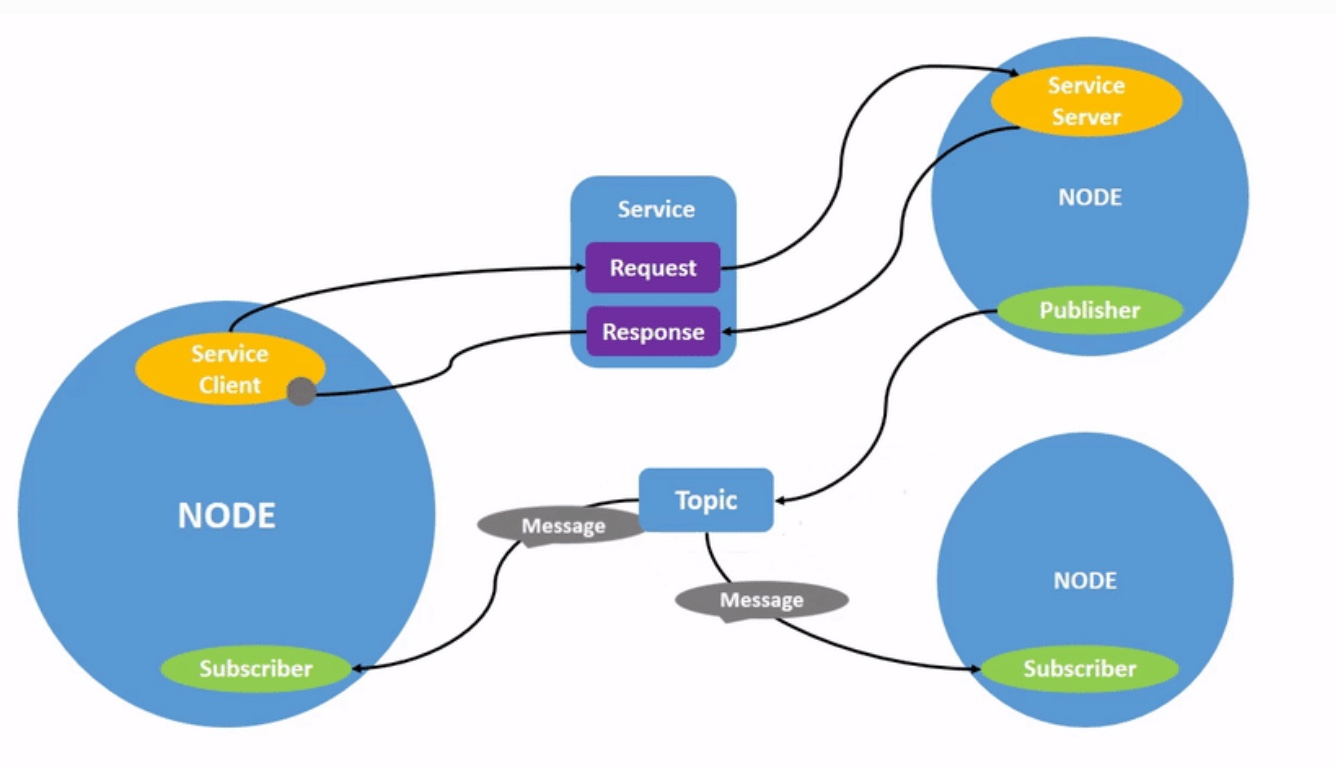
\includegraphics[width=0.75\linewidth]{Img/node.jpg}
    \caption{Nodes}\label{f:node}
    \vspace{-0.1in}
\end{figure}

\subsubsection{Initialization}
\textbf{1. Create a node with default configuration:}
\begin{lstlisting}[language=Python, caption=Python example]
    // Initialize micro-ROS allocator
    rcl_allocator_t allocator = rcl_get_default_allocator();
    
    // Initialize support object
    rclc_support_t support;
    rcl_ret_t rc = rclc_support_init(&support, argc, argv, &allocator);
    
    // Create node object
    rcl_node_t node;
    const char * node_name = "test_node";
    
    // Node namespace (Can remain empty "")
    const char * namespace = "test_namespace";
    
    // Init default node
    rc = rclc_node_init_default(&node, node_name, namespace, &support);
    if (rc != RCL_RET_OK) {
        ... // Handle error
        return -1;
    }
\end{lstlisting}

\textbf{2. Create a node with custom options:} The configuration of the node will also be applied to its future elements (Publishers, subscribers, services, \dots). The API used to customize the node options differs between ROS2 distributions:

Foxy: The \api{rcl\_node\_options\_t} is used to configure the node
\begin{lstlisting}[language=Python, caption=Python example]
// Initialize allocator and support objects
...

// Create node object
rcl_node_t node;
const char * node_name = "test_node";

// Node namespace (Can remain empty "")
const char * namespace = "test_namespace";

// Get default node options and modify them
rcl_node_options_t node_ops = rcl_node_get_default_options();

// Set node ROS domain ID to 10
node_ops.domain_id = (size_t)(10);

// Init node with custom options
rc = rclc_node_init_with_options(&node, node_name, namespace, &support, &node_ops);

if (rc != RCL_RET_OK) {
... // Handle error
return -1;
}
\end{lstlisting}

Galactic: In this case, the node options are configured on the \api{rclc\_support\_t} object with a custom API
\begin{lstlisting}[language=Python, caption=Python example]
// Initialize micro-ROS allocator
rcl_allocator_t allocator = rcl_get_default_allocator();

// Initialize and modify options (Set DOMAIN ID to 10)
rcl_init_options_t init_options = rcl_get_zero_initialized_init_options();
rcl_init_options_init(&init_options, allocator);
rcl_init_options_set_domain_id(&init_options, 10);

// Initialize rclc support object with custom options
rclc_support_t support;
rclc_support_init_with_options(&support, 0, NULL, &init_options, &allocator);

// Create node object
rcl_node_t node;
const char * node_name = "test_node";

// Node namespace (Can remain empty "")
const char * namespace = "test_namespace";

// Init node with configured support object
rclc_node_init_default(&node, node_name, namespace, &support);

if (rc != RCL_RET_OK) {
... // Handle error
return -1;
}
\end{lstlisting}

\textbf{3. Cleaning up:} To destroy a initialized node all entities owned by the node (Publishers, subscribers, services, \dots) have to be destroyed before the node itself. This will delete the node from ROS2 graph, including any generated infrastructure on the agent (if possible) and used memory on the client.
\begin{lstlisting}[language=Python, caption=Python example]
// Destroy created entities (Example)
rcl_publisher_fini(&publisher, &node);
...

// Destroy the node
rcl_node_fini(&node);
\end{lstlisting}

% - NOTE: 
\subsection{Publishers and subscribers}
ROS 2 publishers and subscribers are the basic communication mechanism between nodes using topics. Ready to use code related to this concepts can be found in \href{https://github.com/micro-ROS/micro-ROS-demos/blob/foxy/rclc/int32_publisher/main.c}{micro-ROS-demos/rclc/int32\_publisher} and \href{https://github.com/micro-ROS/micro-ROS-demos/blob/foxy/rclc/int32_subscriber/main.c}{micro-ROS-demos/rclc/int32\_subscriber} folders. Fragments of code from this examples are used on this tutorial. ROS 2 breaks complex systems down into many modular nodes. Topics are a vital element of the ROS graph that act as a bus for nodes to exchange messages.
\begin{figure}[htb!]
    \centering
    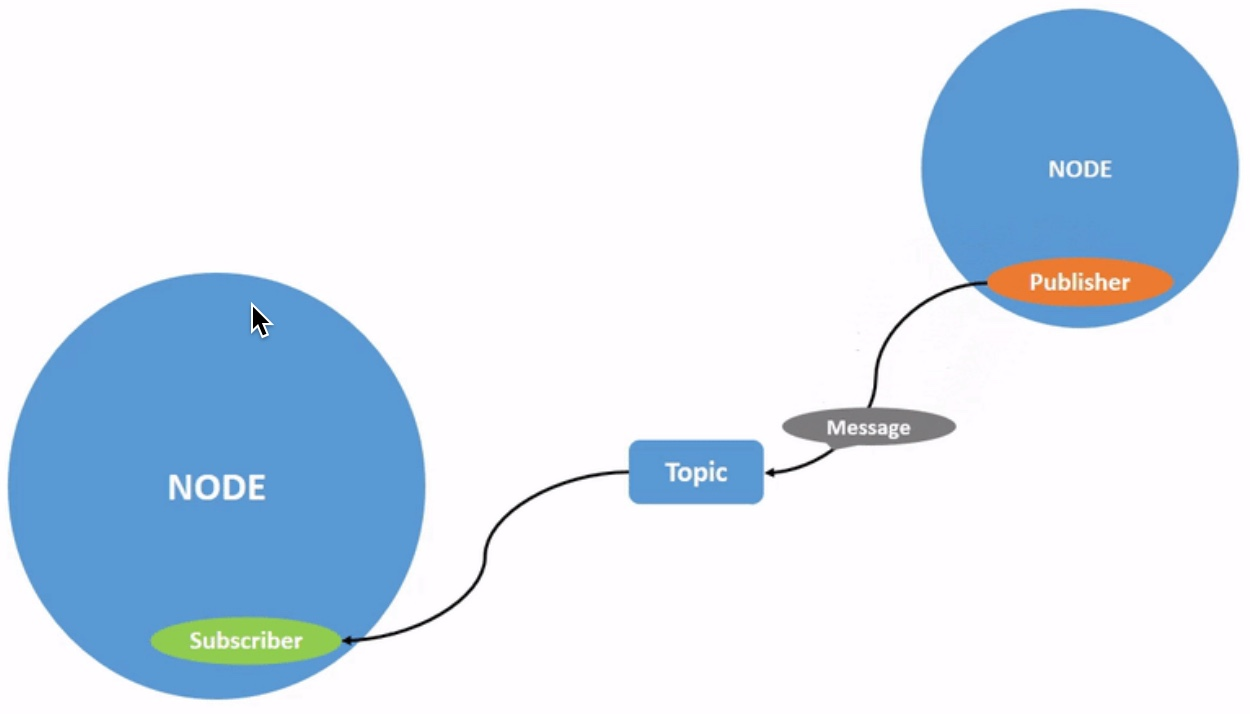
\includegraphics[width=0.55\linewidth]{Img/topic.jpg}
    \caption{Publishers and subscribers}\label{f:topic}
    \vspace{-0.1in}
\end{figure}

A node may publish data to any number of topics and simultaneously have subscriptions to any number of topics. Topics are one of the main ways in which data is moved between nodes and therefore between different parts of the system.
\begin{figure}[htb!]
    \centering
    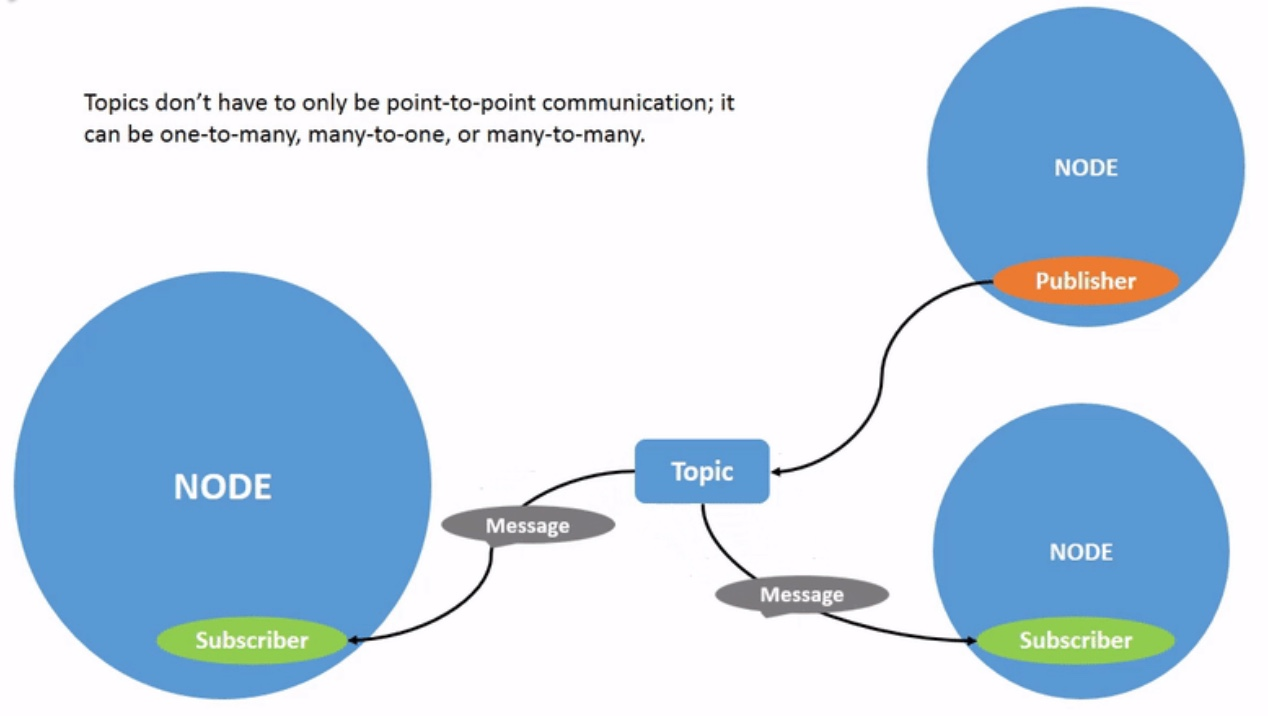
\includegraphics[width=0.55\linewidth]{Img/topic2.jpg}
    \caption{Publishers and subscribers}\label{f:topic2}
    \vspace{-0.1in}
\end{figure}

\subsubsection{Publisher}
\textbf{1. Initialization:} Starting from a code where RCL is initialized and a micro-ROS node is created, there are tree ways to initialize a publisher depending on the desired quality-of-service configuration. For a detail on the available QoS options and the advantages and disadvantages between reliable and best effort modes, check the \href{https://micro.ros.org/docs/tutorials/programming_rcl_rclc/qos/}{QoS tutorial}.

\begin{lstlisting}[language=Python, caption=Reliable (default)]
    // Publisher object
    rcl_publisher_t publisher;
    const char * topic_name = "test_topic";
    
    // Get message type support
    const rosidl_message_type_support_t * type_support =
        ROSIDL_GET_MSG_TYPE_SUPPORT(std_msgs, msg, Int32);
    
    // Creates a reliable rcl publisher
    rcl_ret_t rc = rclc_publisher_init_default(
        &publisher, &node,
        &type_support, &topic_name);
    
    if (RCL_RET_OK != rc) {
        ...  // Handle error
        return -1;
    }
\end{lstlisting}

\begin{lstlisting}[language=Python, caption=Best effort]
    // Publisher object
    rcl_publisher_t publisher;
    const char * topic_name = "test_topic";
    
    // Get message type support
    const rosidl_message_type_support_t * type_support =
        ROSIDL_GET_MSG_TYPE_SUPPORT(std_msgs, msg, Int32);
    
    // Creates a best effort rcl publisher
    rcl_ret_t rc = rclc_publisher_init_best_effort(
        &publisher, &node,
        &type_support, &topic_name);
    
    if (RCL_RET_OK != rc) {
        ...  // Handle error
        return -1;
    }
\end{lstlisting}

\begin{lstlisting}[language=Python, caption=Custom QoS]
    // Publisher object
    rcl_publisher_t publisher;
    const char * topic_name = "test_topic";
    
    // Get message type support
    const rosidl_message_type_support_t * type_support =
        ROSIDL_GET_MSG_TYPE_SUPPORT(std_msgs, msg, Int32);
    
    // Set publisher QoS
    const rmw_qos_profile_t * qos_profile = &rmw_qos_profile_default;
    
    // Creates a rcl publisher with customized quality-of-service options
    rcl_ret_t rc = rclc_publisher_init(
        &publisher, &node,
        &type_support, &topic_name, qos_profile);
    
    if (RCL_RET_OK != rc) {
        ...  // Handle error
        return -1;
    }
\end{lstlisting}

\textbf{2. Publish a message:} Use \api{rcl\_publish} to publish messages to the topic. For periodic publications, \api{rcl\_publish}\footnote{Note that \api{rcl\_publish} is thread safe and can be called from multiple threads.} can be placed inside a timer callback. Check the \href{https://micro.ros.org/docs/tutorials/programming_rcl_rclc/executor/}{Executor and timers section} for details.

\begin{lstlisting}[language=Python, caption=publish messages]
    // Int32 message object
    std_msgs__msg__Int32 msg;
    
    // Set message value
    msg.data = 0;
    
    // Publish message
    rcl_ret_t rc = rcl_publish(&publisher, &msg, NULL);
    
    if (rc != RCL_RET_OK) {
        ...  // Handle error
        return -1;
    }
\end{lstlisting}


\subsubsection{Subscriber}
\textbf{1. Initialization:} The subscription initialization is almost identical to the publisher one:

\begin{lstlisting}[language=Python, caption=Reliable (default)]
    // Subscription object
    rcl_subscription_t subscriber;
    const char * topic_name = "test_topic";
    
    // Get message type support
    const rosidl_message_type_support_t * type_support =
        ROSIDL_GET_MSG_TYPE_SUPPORT(std_msgs, msg, Int32);
    
    // Initialize a reliable subscriber
    rcl_ret_t rc = rclc_subscription_init_default(
        &subscriber, &node,
        &type_support, &topic_name);
    
    if (RCL_RET_OK != rc) {
        ...  // Handle error
        return -1;
    }
\end{lstlisting}

\begin{lstlisting}[language=Python, caption=Best effort]
    // Subscription object
    rcl_subscription_t subscriber;
    const char * topic_name = "test_topic";
    
    // Get message type support
    const rosidl_message_type_support_t * type_support =
        ROSIDL_GET_MSG_TYPE_SUPPORT(std_msgs, msg, Int32);
    
    // Initialize best effort subscriber
    rcl_ret_t rc = rclc_subscription_init_best_effort(
        &subscriber, &node,
        &type_support, &topic_name);
    
    if (RCL_RET_OK != rc) {
        ...  // Handle error
        return -1;
    }
\end{lstlisting}

\begin{lstlisting}[language=Python, caption=Custom QoS]
    // Subscription object
    rcl_subscription_t subscriber;
    const char * topic_name = "test_topic";
    
    // Get message type support
    const rosidl_message_type_support_t * type_support =
        ROSIDL_GET_MSG_TYPE_SUPPORT(std_msgs, msg, Int32);
    
    // Set client QoS
    const rmw_qos_profile_t * qos_profile = &rmw_qos_profile_default;
    
    // Initialize a subscriber with customized quality-of-service options
    rcl_ret_t rc = rclc_subscription_init(
        &subscriber, &node,
        &type_support, &topic_name, qos_profile);
    
    if (RCL_RET_OK != rc) {
        ...  // Handle error
        return -1;
    }
\end{lstlisting}

\textbf{2. Callbacks:} The executor is responsible to call the configured callback when a message is published. The function will have the message as its only argument, containing the values sent by the publisher:
\begin{lstlisting}[language=Python, caption=Sub-callback decalaration]
    // Function prototype:
    void (* rclc_subscription_callback_t)(const void *);
    
    // Implementation example:
    void subscription_callback(const void * msgin)
    {
        // Cast received message to used type
        const std_msgs__msg__Int32 * msg = (const std_msgs__msg__Int32 *)msgin;
    
        // Process message
        printf("Received: %d\n", msg->data);
    }
\end{lstlisting}

Once the subscriber and the executor are initialized, the subscriber callback must be added to the executor to receive incoming publications once its spinning:
\begin{lstlisting}[language=Python, caption=Sub-callback registration]
    // Message object to receive publisher data
    std_msgs__msg__Int32 msg;
    
    // Add subscription to the executor
    rcl_ret_t rc = rclc_executor_add_subscription(
        &executor, &subscriber, &msg,
        &subscription_callback, ON_NEW_DATA);
    
    if (RCL_RET_OK != rc) {
        ...  // Handle error
        return -1;
    }
    
    // Spin executor to receive messages
    rclc_executor_spin(&executor);
\end{lstlisting}

\subsubsection{Message initialization}
Before publishing or receiving a message, it may be necessary to initialize its memory for types with strings or sequences. Check the \href{https://micro.ros.org/docs/tutorials/advanced/handling_type_memory/}{Handling messages memory in micro-ROS} section for details.

\subsubsection{Cleaning Up}
After finishing the publisher/subscriber, the node will no longer be advertising that it is publishing/listening on the topic. To destroy an initialized publisher or subscriber:
\begin{lstlisting}[language=Python, caption=To destroy an initialized publisher or subscriber]
// Destroy publisher
rcl_publisher_fini(&publisher, &node);

// Destroy subscriber
rcl_subscription_fini(&subscriber, &node);
\end{lstlisting}





% - NOTE: Services
\subsection{Services}
Services are another method of communication for nodes in the ROS graph. Services are based on a call-and-response model, versus topics’ publisher-subscriber model. While topics allow nodes to subscribe to data streams and get continual updates, services only provide data when they are specifically called by a client. Ready to use code related to this concepts can be found in \href{https://github.com/micro-ROS/micro-ROS-demos/blob/foxy/rclc/addtwoints_server/main.c}{micro-ROS-demos/rclc/addtwoints\_server} and \href{https://github.com/micro-ROS/micro-ROS-demos/blob/foxy/rclc/addtwoints_client/main.c}{micro-ROS-demos/rclc/addtwoints\_client} folders. Fragments of code from this examples are used on this tutorial.
\begin{figure}[htb!]
    \centering
    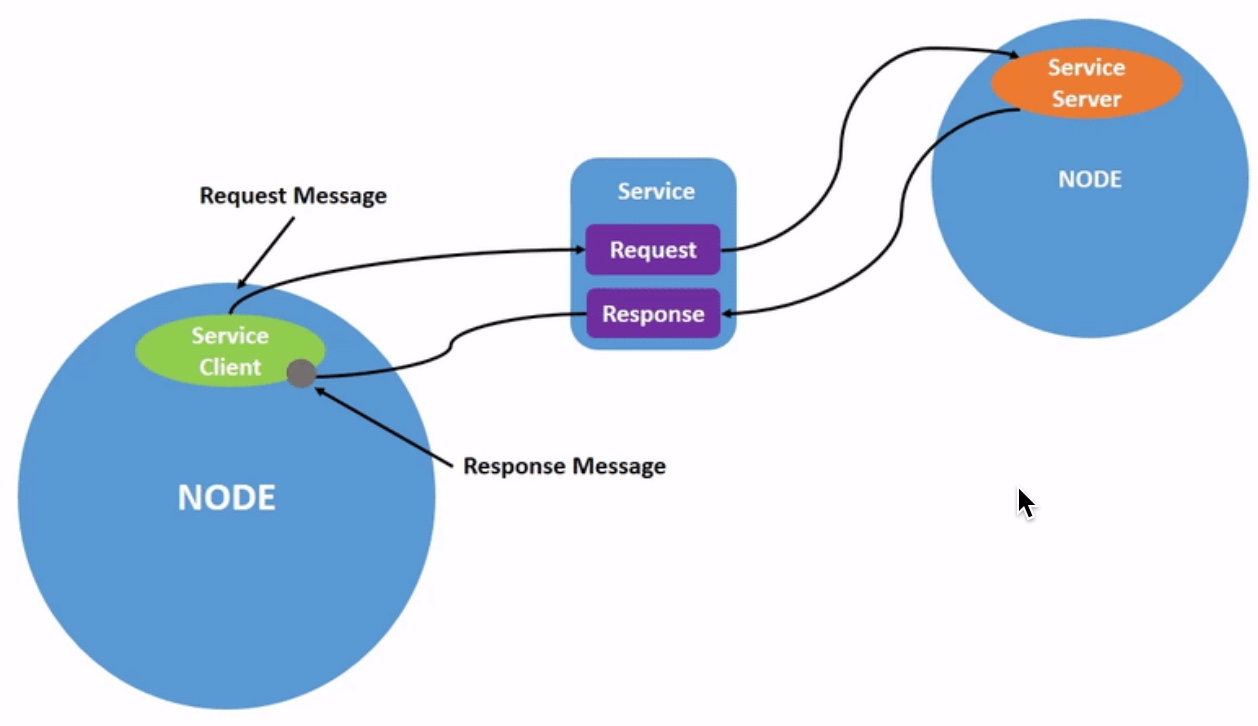
\includegraphics[width=0.75\linewidth]{Img/service1.jpg}
    \caption{Service}
    \vspace{-0.1in}
\end{figure}
\begin{figure}[htb!]
    \centering
    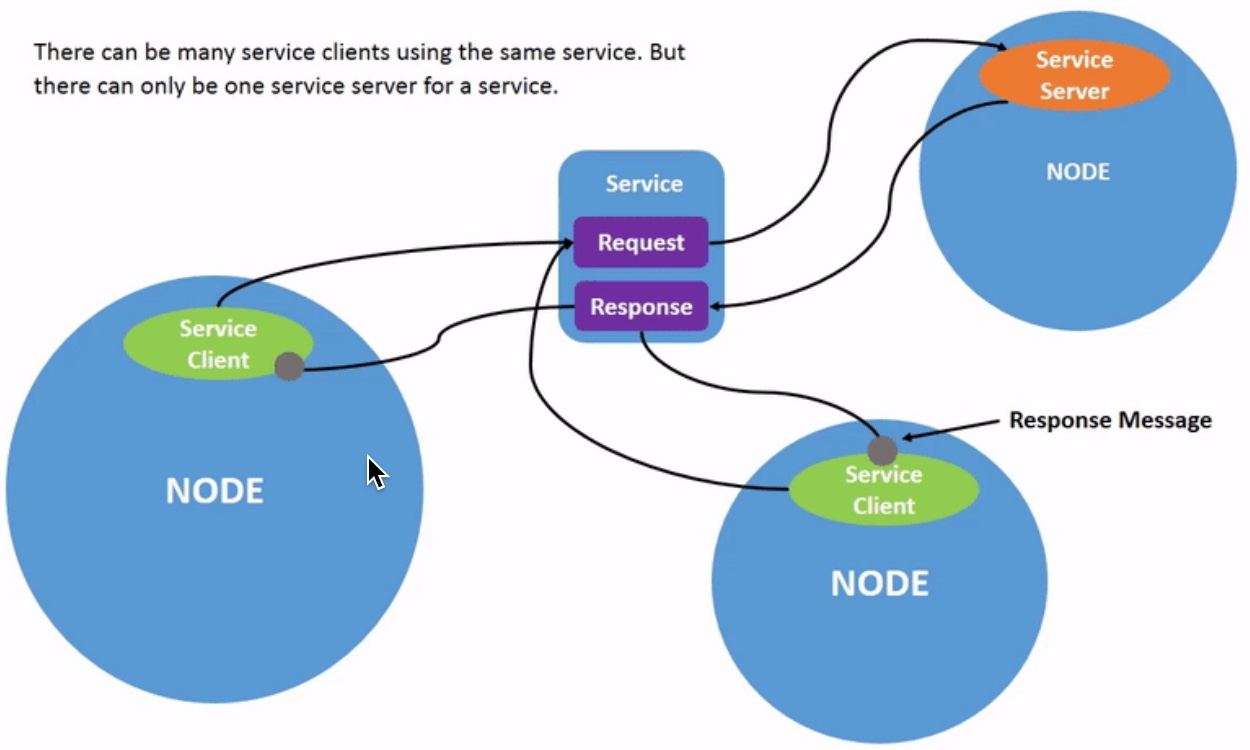
\includegraphics[width=0.75\linewidth]{Img/service2.jpg}
    \caption{Service2}
    \vspace{-0.1in}
\end{figure}

\todo{https://micro.ros.org/docs/tutorials/programming\_rcl\_rclc/service/}
\subsubsection{Service server}
\subsubsection{Service Client}
\subsubsection{Message initialization}
\subsubsection{Cleaning Up}


\subsection{Parameter server}
\todo{https://micro.ros.org/docs/tutorials/programming\_rcl\_rclc/parameters/}

\subsection{Executor and timers}
\subsubsection{Timer}
Timers can be created and added to the executor, which will call the timer callback periodically once it is spinning. They are usually used to handle periodic publications or events.

\textbf{1. Initialization:}
\begin{lstlisting}[language=Python, caption=Timer Initialization]
    // Timer period on nanoseconds
    const unsigned int timer_period = RCL_MS_TO_NS(1000);
    // Create and initialize timer object
    rcl_timer_t timer;
    rcl_ret_t rc = rclc_timer_init_default(&timer, &support, timer_period, timer_callback);
    // Add to the executor
    rc = rclc_executor_add_timer(&executor, &timer);
    if (rc != RCL_RET_OK) {
        ... // Handle error
        return -1;
    }    
\end{lstlisting}

\textbf{2. Callback:} The callback gives a pointer to the associated timer and the time elapsed since the previous call or since the timer was created if it is the first call to the callback. During the callback the timer can be canceled or have its period and/or callback modified using the passed pointer. Check rcl/timer.h for details.
\begin{lstlisting}[language=Python, caption=Timer Callback]
    void timer_callback(rcl_timer_t * timer, int64_t last_call_time)
    {
        printf("Last callback time: %ld\n", last_call_time);
    
        if (timer != NULL) {
            // Perform actions
            ...
        }
    }  
\end{lstlisting}

\textbf{3. Cleaning Up:} To destroy an initialized timer, This will deallocate used memory and make the timer invalid.
\begin{lstlisting}[language=Python, caption=Timer Cleaning up]
    // Destroy timer
    rcl_timer_fini(&timer);
    This will deallocate used memory and make the timer invalid    
\end{lstlisting}



\subsubsection{Executor}

\subsection{Quality of service}

\subsection{micro-ROS utilities}

\section{Data Distribution Service (DDS)}
\textbf{DDS itself is an API specification and the actual underlying protocol is the Real-Time Publish-Subscribe Protocol (RTPS)\cite{RTPS}.} Multiple open-source implementations of DDS are available for full-fledged computers running Linux or Windows. Few implementations are suitable for resource-constrained embedded systems.

eProsima FastRTPS is a popular RTPS implementation that is also the underlying middleware for ROS 2. OpenDDS is another widespread implementation that is a DDS implementation on top of the RTPS protocol~\cite{OpenDDS}. Real-Time Innovations (RTI) offers ConnextDDS, a commercial DDS implementation~\cite{ConnextDDS}. All of the implementations mentioned above target Linux, Windows or MacOS and do not run on embedded platforms. RTI also offers microDDS, an implementation suitable for microcontrollers. In contrast to embeddedRTPS~\cite{kampmann2019portable}, microDDS is not open source and only commercially available. Lastly, freeRTPS 2 is an implementation originally developed for microcontrollers in the context of ROS 2. This implementation explicitly targets STM32 microprocessors and is not under active maintenance.

The DDS Extremely Resource Constrained Environments (XRCE) standard is intended for integration of embedded systems into DDS networks~\cite{XRCE}. The resource-constrained platform is integrated into the DDS network by a more powerful server, that acts as a gateway. \textbf{In this architecture, the microcontroller is not an independent, first-class participant in the communication network, as it's ability to communicate depends on server.} This also introduces a single point of failure, rendering this architecture potentially unsuitable for safety-critical applications.

\subsection{Background of RTPS}
This section provides a brief overview of the basic concepts behind RTPS. We cover the basic entities, the discovery procedure and data exchange mechanisms. An exhaustive description is provided in the standard maintained by the OMG~\cite{RTPS}.

\subsubsection{Entities}
As depicted in Fig. \ref{f:rtps}, the basic actors in RTPS are \textit{participants}, which in turn have a variable number of readers or writers. Readers or writers (summarized as \textit{endpoints} in the following) can be identified with an id composed of a unique participant prefix and an entity id which is unique within this participant. They communicate through a publish-subscribe mechanism, a concept also common in other messaging frameworks such as ROS or Message Queuing Telemetry Transport (MQTT). \textbf{Endpoints are loosely coupled only by a topic name and data type definition.} From a user perspective, messages published by writers are addressed to a topic and not to specific recipients. Respectively, readers subscribe to a specific topic and join the network without knowledge about the specific writer(s). For this, participants become aware of each other during runtime in the course of a decentralized discovery process. Thus, readers and writers form a loosely coupled communication network that is suitable for runtime integrated systems.
\begin{figure}[htb!]
    \centering
    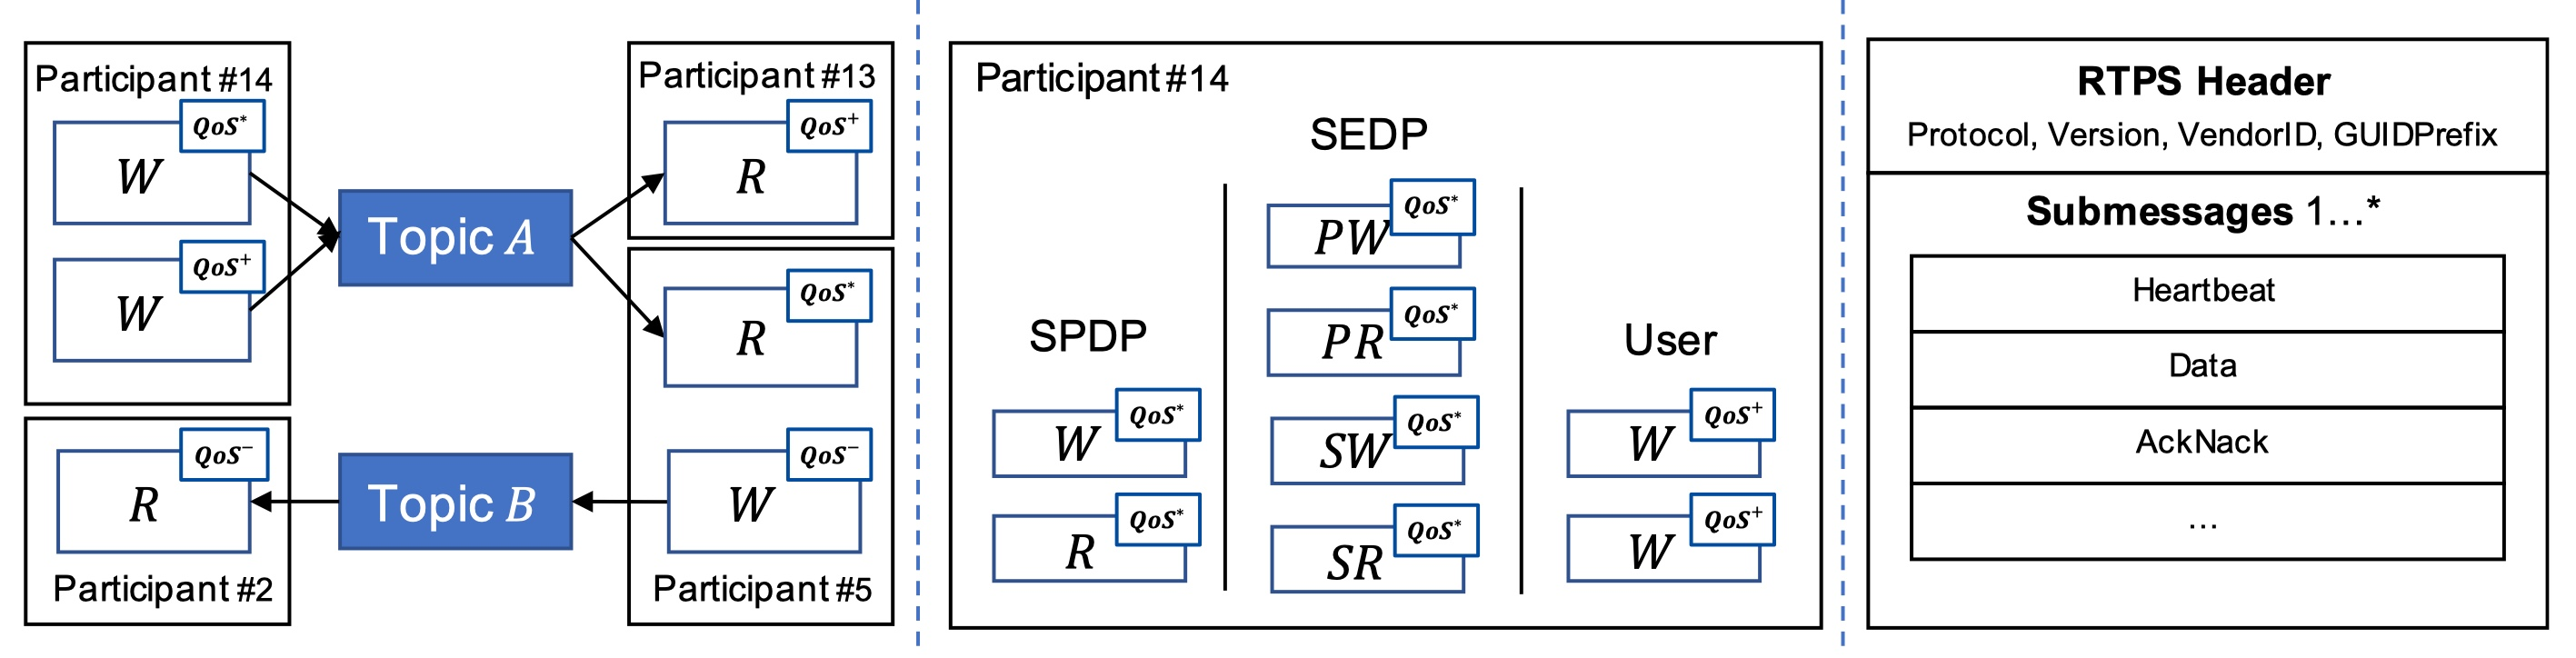
\includegraphics[width=0.95\linewidth]{Img/RTPS.jpg}
    \caption{\text{Left}: Participants Exchange Messages via User-defined Reader and Writer Endpoints. \textbf{Middle}: Built-in RTPS endpoints for Participant (SPDP) and Endpoint Discovery (SEDP) alongside user-defined Endpoints. \textbf{Right}: Components of RTPS Messages encapsulated in UDP Packets.}\label{f:rtps}
    \vspace{-0.1in}
\end{figure}

Various Quality of Service (QoS) parameters can be used to customize the behavior of endpoints. For example, writers and readers communicate either in a \textit{reliable} or \textit{best-effort} mode. \textbf{Reliable writers keep track of already transmitted packages through sequence numbers and are able to resend messages in case of a transmission failure. Best-effort writers do not provide this capability.} The user interacts with endpoints by passing serialized data to writers or receiving data from readers. RTPS is specified for TCP/UDP communication.

In general, endpoints send \underline{UDP packets} that are structured as depicted in Fig. \ref{f:rtps}. Each message starts with a header that contains, among other fields, the RTPS version or vendor identification. The header is followed by a variable amount of sub-messages that are used for data exchange and discovery. \texttt{Data} sub-messages are used to exchange generic, serialized data between readers and writers. \texttt{Heartbeat} and \texttt{AckNack} sub-messages are used to provide a reliable communication. The \texttt{Heartbeat} sub-message allows writers to announce the available sequence numbers in its storage. Reliable readers send \texttt{AckNack} sub-messages to communicate missing as well as received packets. Based on those acknowledgments, the reliable writer can decide when a packet can be safely removed from its history. While one or multiple participants are addressed by a specific port, the target endpoint is identified by the entity id passed with the aforementioned messages.

\subsubsection{Discovery Protocols}
Entities in RTPS discover each other through a decentralized two-step discovery process, using a set of six built-in endpoints as depicted in Fig. \ref{f:rtps}. Technically, these are regular endpoints that function just like user-defined endpoints but communicate specific messages for the discovery process and have a fixed entity id. In the first step, the Simple Participant Discovery Protocol (SPDP) uses a reader/writer pair of best-effort endpoints for discovery of participants and their properties in the network. Each participant periodically sends messages through the SPDP-writer containing information about the participant on standardized IP broadcast addresses. The transmitted UDP packets are made up of RTPS packets containing a \texttt{Data} sub-message and are received by remote SPDP-readers. Discovery of those endpoints is not required because the messages are send on addresses which are relevant for all participants and the destination is known as the built-in endpoints have fixed entity ids. SPDP messages contain, among others, the unicast or multicast locators (i.e. IP-address and port) for meta (e.g. discovery) and user traffic to the sending participant.

Once the participants become aware of each other, they exchange information about user-defined endpoints using the Simple Endpoint Discovery Protocol (SEDP). For this, reliable writers and readers are used. The publication writer PW sends information about user-defined writers to all known participants by addressing the publication readers PR of all known participants. For each user-defined endpoint, information about it’s QoS parameters, locators and their entity id are transmitted. Analogously, user-defined readers are announced through the subscription-writer SW and participants receive these respective messages through the subscription-reader SR. After discovering a new endpoint, a participant tries to match it with one if its own endpoints. Endpoints are matched if the topic name, data type name and QoS parameters are compatible.

Once local endpoints have been matched with remote endpoints, every message that is handed to the writer will be send to all known, matching readers in the network. For this purpose, the user hands over a serialized byte array, that is inserted into RTPS packet containing a \texttt{Data} sub-message. Note that SPDP and SEDP messages are sent periodically, therefore participants and endpoints can dynamically join the RTPS network.